To motivate the course and its objective, consider the following example
from glaciology.

An ice sheet is a large accumulation of ice. The largest ice sheets take
thousands of years to millennia to form. If the climate is stable enough
(say, it is \emph{constant}), the ice sheet may reach a \emph{stable}
\emph{equilibrium}.

This equilibrium results from a balance between \emph{accumulation} of
snow above the \emph{snowline} (which is determined by the external
climate conditions), and the \emph{ablation} of ice that is being pushed
below the snow line.

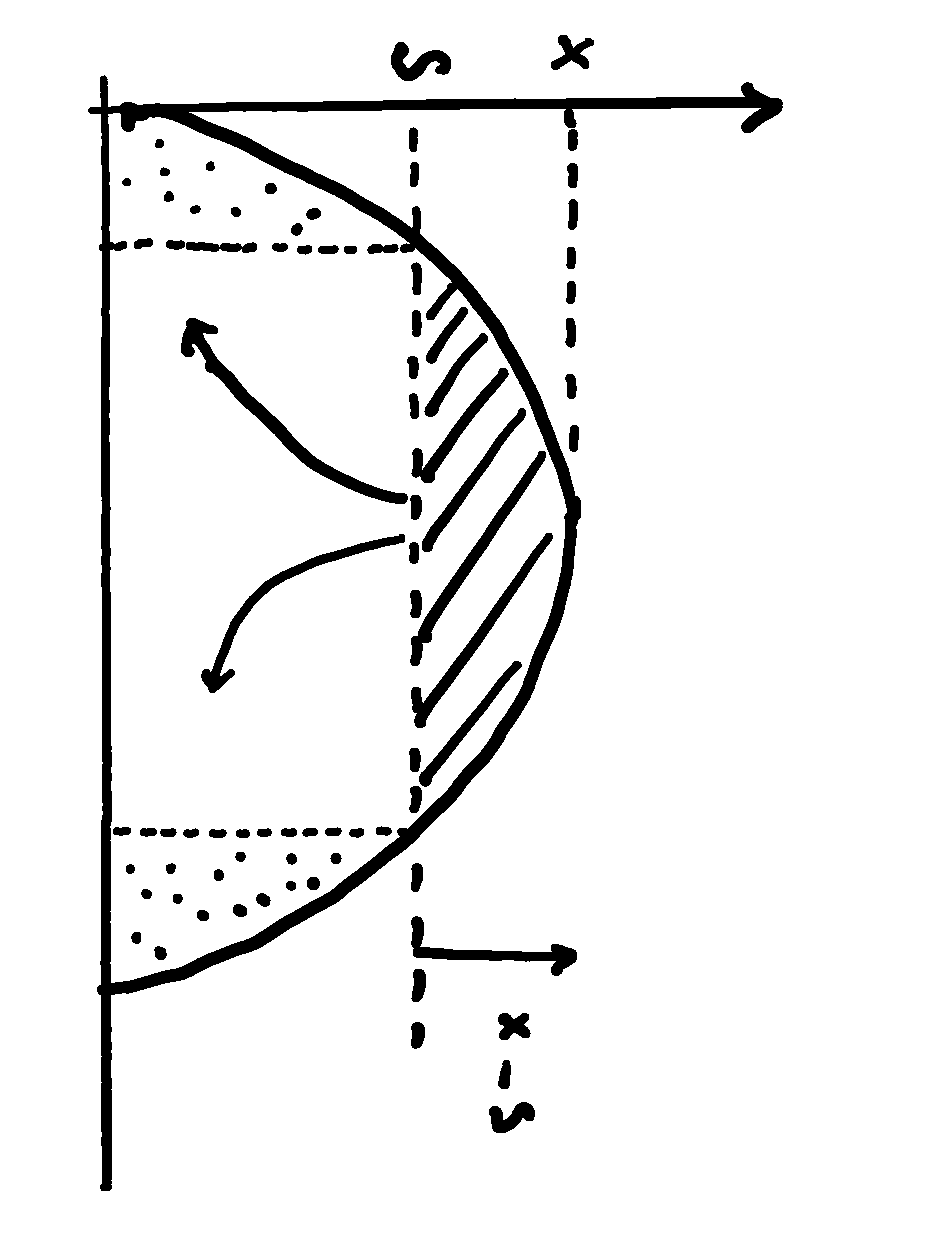
\includegraphics[page=1, angle=90, scale=0.7]{lphys2114-figures}

Intuitively, we may perceive that if climate warms a little, the
altitude of the ice sheet will decrease (implying less net
accumulation), but the flow of ice towards the ice sheet will be reduced
as well, so that a new balance will be reached. However, we may already
anticipate that if the climate warms \emph{too much}, and the top
surface of the ice sheet might drawn under the snowline, at which point
we expect a catastrophic meltdown of the icesheet.

We witness here a non-linear phenomenon. There is what some might call a
\emph{tipping point}, a point of warming above which the qualitative
behaviour of the object changes. In this course, we would like to use
mathematical modelling and a mathematical language to describe this
behaviour, and many others. We will be introduced to the theory and
learn the techniques that allow us to describe the expected behaviour of
such systems.

The standard theory is the theory of \emph{dynamical systems}. In
essence, a dynamical system is the combination of a state space, say
\(\Omega\), and a \emph{rule} that determines the evolution of every
point of the state space.

This is perhaps a bit abstract, so consider again our ice sheet example.

Call the altitude of the summit of the ice sheet \(x\). This is positive
real number, so \(x \in \mathbb{R}^+\). The altitude of the snowline is
\(S\). We consider that it is constant, so in the following we will view
it as a \emph{parameter}.

Here, we have \emph{summarised} the state of our real-world system (the
ice sheet) with a single variable \(x\). That variable evolves in
\(\mathbb{R}^+\). So in our case the \(\Omega\) space is
\(\mathbb{R}^+\). Now we need a rule for the evolution of an ice sheet
that would have an altitude \(x\).

One (standard) approach is to write a \emph{differential equation}.
Simply, we equate \(\dt x\) with a function of the state \(x\), and the
parameter \(S\). At this point, we need a bit of physical intuition.
\(x\) will evolve as a balance between accumulation and ablation. The
difference between accumulation and ablation is called \emph{net
accumulation}. One (simplistic) way of putting it, is that net
accumulation is proportional to the distance between \(x\) and \(S\). It
would be an equation of the kind

\begin{equation}
\ddt x = x - S
\end{equation}

\bcd
Consider an initial condition \(x_0 = x(t_0)\). Finding \(x_t\) for
\(t>t_0\) is an initial value problem, which is a particular case of a
Cauchy problem. Find the solutions. Show that their behaviour differ
depending on the initial condition. Explain also what is wrong with this
model. How can we fix it ? \ecd

After discussion, we see that we need a \emph{negative feedback} to
prevent ice to grow until infinity when it starts above the snowline. We
won't discuss too much the phenomenological details here, but say that
the negative feedback is related to the flow of ice towards the ice
sheet ablation zone, which is enhanced when the ice sheet grows very
big. So our final equation would resemble:

\begin{equation}\label{eq:icesheetmodel}
\ddt x = x -  a x^2 - S\text{ if }x>0\text{, and }\dt x = \text{max}(0, -S)\text{ if }x=0, 
\end{equation}

where \(a\) is a parameter. Again, we look after qualitative behaviours,
and for (mathematical) simplicity we will set \(a=1/4\). In practice we
cannot be so relaxed about fixing parameters, but this is for the sake
of the demonstration.

What is going on now ?

\bcd
A fixed point \(x_f\) of the differential equation is an element of the
domain \(\Omega\) such that the system is invariant at that point. That
is, if \(x(t_0)=x_f\) for a given \(t=t_0\), then \(x(t)=x_f\) for any
time \(t\) of the time domain. How do you find the fixed points
associated with the dynamical system in \eqref{eq:icesheetmodel} ? \ecd 

After discussion, we find that the number of fixed points depends on the
value of the parameter \(S\): one fixed point for \(S<0\)
\(2(1+\sqrt(1-S))\), one fixed point for \(S>1\) (x=0), and three fixed
points between these values (which ones ?)

\includegraphics[page=2, angle=90, scale=0.7]{lphys2114-figures}

Now we would like to determine the behaviour of the system for initial
conditions between these points. One approach would be to resolve the
ordinary differential equation \eqref{eq:icesheetmodel}. For \(S=0\) it
is doable (hint: use the separation of variables: put all \(\dif x\)
terms on one side; the \(\dif t\) terms on the other side; integrate and
solve for \(x\)) but it is cumbersome and the strategy will actually not
work in most cases. In other words, most non-linear ordinary
differential equations have no analytical solutions.

Hence, a more fruitful strategy is to study the behaviour of \((t)\)
\emph{near} (in French: \emph{dans le voisinage the}) fixed points, and
use theory to connect the flowlines between fixed points.

The model we have been starting with is of the form
\(\ddt x = F (x;\psi)\) with, here, \(\psi := \{S\}\). By definition of
a fixed point, \(F(x_f;\Psi)=0\) (the dependency on \$psi\$ is dropped
for clarity). Define \(\delta x := x-x_f\).

\begin{equation}
\ddt {x-x_f} \eqbdef \ddt {\delta_x} = \underbrace {\left.\pd{F(x;\psi)}{x}\right|_{x_f}}_{\lambda}  \delta x + \mathcal{O}(x^2)
\end{equation}

This is a linear differential equation for \(\delta x\) with constant
coefficient. That is, near enough to the fixed point, \(\delta x\)
decays (if \(\lambda < 0\)) or grows (if \(\lambda > 0\)) exponentially
with e-folding time \(1/\lambda\). This distinguishes a point that is
\emph{locally stable} from a point that is \emph{locally unstable}.

\bcd
Reconsiders the one to three solutions of the bifurcation diagram. Which
ones are stable, and which one unstable ? What we see appearing are
\emph{stable} and \emph{unstable} solution \emph{branches}. \ecd 

\includegraphics[page=3, angle=90, scale=0.7]{lphys2114-figures}

Hence, even though we have avoided to resolve the ordinary differential
equation; (we have avoided to solve the initial value problem), but
provided that we have identified all fixed points, and characterised
their local stability, we have gained a good qualitative picture of the
system's behavior. For any value of \(S\), we can picture the
\emph{flow} associated with the dynamical system, that is, for any point
\(x\) of the domain \(\Omega\), we know the direction taken by \(x\) as
time progresses.

This is an example of qualitative analysis of a non-linear dynamical
system, which, as we see it here, is reasonably simple but not
simplistic. We have identified \emph{invariant sets}, that is, sets of
points that are left unchanged by the flow. In this example, invariant
sets are fixed points. We have identified \emph{bifurcation points},
that is, points of the parameter space \(S\) where the number or the
stability of the invariant sets (again, here, fixed points).

In this first lecture, meant to motivate the course, we have been
informal and did not justify our findings with theorems; nor did we
attempt to be too systematic and rigorous with definitions. But we
understand our objectives: identify the nature of invariant sets,
estimate their stability, and depict the behaviour of the system between
these invariant sets.

Specifically, the lecture will be divided into two broad sections:

\begin{itemize}
\tightlist
\item
  continuous dynamical systems (expressed as ordinary differential
  equations)
\item
  discrete dynamical systems (expressed as iterations)
\end{itemize}

Dynamical systems will be deterministic (but informally, from time to
time I will mention the interest and possibilities brought about by
stochastic dynamical systems), and we will not go beyond three
dimensions.
